\documentclass[11pt, a4paper, twocolumn]{article}

% Fonts and math (Elsevier-like Times style)
\usepackage{graphicx} % Required for inserting images
\usepackage{array} % For extra column formatting
\usepackage{amsmath, amssymb, cancel, siunitx, mathtools, physics2, upgreek} % for equation environment
\usepackage{float,geometry,subcaption,tikz,circuitikz}
\geometry{margin=2cm}
\usepackage[skip=10pt]{parskip}
\usepackage{setspace}
\usepackage{hyperref, cleveref}
\usepackage{cite, bookmark}
\usepackage{url}
\usepackage[table,xcdraw]{xcolor}
\usepackage[export]{adjustbox}
\usepackage{listings,pdfpages}
\usepackage{dblfloatfix}

% --- Abstract styling (elsarticle look)
\usepackage{abstract}
\renewcommand{\abstractnamefont}{\normalfont\bfseries}
\renewcommand{\abstracttextfont}{\normalfont}
\renewenvironment{abstract}{%
  \par\noindent\rule{\linewidth}{0.4pt}\par
  \begin{center}\bfseries Abstract\end{center}%
}{%
  \par\rule{\linewidth}{0.4pt}\par
}

% --- Section styling (similar to elsarticle
\usepackage{titlesec}
\titleformat{\section}{\normalfont\large\bfseries}{\thesection.}{0.5em}{}
\titleformat{\subsection}{\normalfont\normalsize\bfseries}{\thesubsection.}{0.5em}{}

% Table of contents styling
\usepackage{tocloft}
\cftsetindents{section}{0em}{2em}
\cftsetindents{subsection}{1em}{2em}
\renewcommand\cfttoctitlefont{\hfill\Large\bfseries}
\renewcommand\cftaftertoctitle{\hfill\mbox{}}
\renewcommand\cftfigfont{\footnotesize}
\renewcommand\cftfigpagefont{\footnotesize}
\renewcommand\cftloftitlefont{\large}

\graphicspath{ {./images/} }

\definecolor{blurple}{HTML}{5865F2}
\definecolor{backcolour}{HTML}{272823}

\hypersetup{
    colorlinks=true,
    linkcolor=black,
    urlcolor=black,
    citecolor=blurple,
}

\urlstyle{same}

\DeclareMathOperator{\sinc}{sinc}

\renewcommand{\arraystretch}{1.4}

% Python code export
\lstset{
    language=Python,
    basicstyle=\ttfamily\scriptsize,
    keywordstyle=\color{magenta},       
    commentstyle=\color{gray},        
    stringstyle=\color{teal},  
    showstringspaces=false,
    frame=single,
    breaklines=true,
    numbers=left,
    numberstyle=\tiny\color{gray}
}

\setcounter{secnumdepth}{5}
\setcounter{tocdepth}{5}

\hbadness=99999

%%%%%%%%%%%%%%%%%%%%%%%%%%%%%%%%%%%

\title{%


\includegraphics[width=0.2\linewidth]{ucd_brandmark_black.jpg} \vspace{0.5cm}\\

{\Large\bfseries UCD School of Physics}\vspace{1.5cm}\\

{\large PHYC30170 Physics Astronomy and Space Lab I}\\
{\bfseries Skin Depth}

}
\author{Joana C.C. Adao \\ \small Student No.: 23311051}
\date{\today}

\begin{document}

% Title page - single column
\onecolumn
\maketitle

% Abstract - single column
\pagenumbering{roman}
\setcounter{page}{1}
\begin{abstract}

This experiment sought to investigate the skin depth phenomenon and frequency-dependence of it in cylindrical conductors of copper, aluminium, brass, and steel. By measuring the induced voltage and time lag across the conductors over a frequency range of 5 to 62 kHz, the electrical conductivity ($\sigma$) was determined for all metals and the relative permeability ($\mu_r$) was determined for the steel sample. The experiment results verified the linear relationship between the induced voltage ratio ($V/f$) and the inverse square root of the frequency ($f^{-1/2}$) within mid-range frequencies. The calculated conductivity for the copper was found to be (5.31 ± 1.58) $\times$\num{e7} S/m, showing strong agreement with the literature value of \num{5.96e7} S/m. Discrepancies in the values for the aluminium and brass from the expected values were observed with (1.62 ± 0.34) $\times$\num{e7} S/m and (6.46 ± 1.12) $\times$\num{e6} S/m respectively, likely due to alloy compositions or apparatus calibration errors. For the ferromagnetic steel rod, a decoupling of equations was used to isolated and calculate the conductivity (\num{1.31e6} S/m) and relative permeability (95.90), values that are more consistent with carbon or alloy steels.

\end{abstract}

\newpage

% Table of Contents - single column
\tableofcontents

\newpage

%%%%%%%%%%%%%%%%%%%%%%%%%%%%%%%%%%%

% Start main content in two columns
\twocolumn
\pagenumbering{arabic}
\setcounter{page}{1}

\section{Introduction} \label{sec:1}

The electromagnetic phenomenon known as the skin depth or skin effect is present in everyday electrical equipments and materials. The name "skin depth" came from the behaviour of current gathering on the outer surface of a conductor, acting like a sort-of skin. It is the tendency of magnetic flux and alternating currents of high-frequency to penetrate the conductor to this limited skin-like depth. The depth of penetration is dependent on frequency and innate material properties such as conductivity or resistivity, and permeability. The skin depth dominates at radio frequencies, and at higher-frequencies of alternating current for a thick rod, it becomes a surface phenomenon rather than a volume phenomenon. \cite{wheeler2006formulas,app132212416}

\section{Theory} \label{sec:2}

\subsection{Eddy Currents}

Physically, the skin effect originates from the induction of eddy currents in the conductor material. A time-varying magnetic field $ \mathbf{B}_{\text{ext}} = \mathbf{B}_0 e^{i \omega t} $ is generated in a material where an alternating current is applied. Eddy currents are generated following Faraday's law of induction \cite{griffiths2023introduction}:

\begin{equation*}
  \nabla \times \mathbf{E} = - \frac{\partial \mathbf{B}}{\partial t}
\end{equation*}

The changing flux defined here induces an electrical field within the conducting material, which drives the eddy currents of current density $ \mathbf{J} = \sigma \mathbf{E} $. As per Lenz's law, these eddy currents generate also their own magnetic fields $ \nabla \times \mathbf{B} = \mu \mathbf{J} $. These equations give and include the electrical conductivity $ \sigma $ and the magnetic permeability $ \mu $. \cite{griffiths2023introduction}

Lenz's law also states that these secondary generated magnetic fields oppose the primary external magnetic field. Inside the conductor, these fields mostly cancel each other, though this cancellation lessens nearer the surface of the material. This relationship is what generates the "skin" at the surface where the current and flux are confined too, effectively shielding the interior. \cite{griffiths2023introduction}

\subsection{Magnetic Field \& Skin Depth}

From Maxwell's equations, a diffusion equation may be derived for a linear and isotropic conductor \cite{griffiths2023introduction}:

\begin{equation*}
  \nabla^2 \mathbf{B} = \mu\sigma \frac{\partial \mathbf{B}}{\partial t}
\end{equation*}

When a high-frequency field enters a conductor and propagates through it, the solution for this equation follows the exponential decay of the magnetic amplitude $B(x)$ at a depth $x$ \cite{griffiths2023introduction,knoepfel2008magnetic},

\begin{equation*}
  B(x) = B_0 e^{-x/\delta}
\end{equation*}

The skin depth $\delta$ is defined here as the distance to which the field amplitude falls to $1/e$ or about $\sim 37\%$ of the surface amplitude. The skin depth is given by \cite{wheeler2006formulas,knoepfel2008magnetic},

\begin{equation} \label{eq:1}
  \delta = \sqrt{\frac{2}{\omega \mu \sigma}} = \frac{1}{\sqrt{\pi f \mu \sigma}}
\end{equation}

Here also $\mu$ is magnetic permeability ($\mu_0\mu_r$) and $\sigma$ is electrical conductivity, $f$ is frequency and $\omega$ the angular frequency. As frequency increases, the skin depth $\delta$ decreases with the relationship $\delta \propto 1/\sqrt{f}$, which confines the fields to a narrow region. \cite{wheeler2006formulas,wiederick,ziolkowska,knoepfel2008magnetic}

\subsection{Induced Voltage}

For an experiment in which a conducting rod of radius $R$ is inserted inside of a solenoid, called the pick-up coil, the magnetic flux $\Phi$ is concentrated only in the region it can penetrate. By Faraday's law of induction, the total flux across the rod is given by the integral of the field. For the "strong skin effect" limit ($R \gg \delta$), the induced voltage in the secondary (pick-up) coil of n turns is given with \cite{wiederick},

\begin{equation*}
  V = - n \frac{d \Phi}{d t}
\end{equation*}

The effective magnetic field inside the conductor is governed by the penetration depth (skin depth) $\delta$, and at the high-frequencies for which there is the strong skin effect, the electrical field contribution scales with $\delta$, $V \propto \omega\delta$, which can be . \cite{wiederick}

With \autoref{eq:1}, this relationship can be expressed in terms of frequency $V/f \propto f^{-1/2}$, which gives the linearised relationship \cite{wiederick}:

\begin{equation} \label{eq:2}
  \frac{V}{f} = a + bf^{-1/2}
\end{equation}

By plotting $V/f$ against $f^{-1/2}$, the slope (a), which accounts for the external field and geometric constants, the conductivity of the material can be measured, provided the permeability is known. Constant (b) accounts for $\mu$, $\sigma$, and coil geometry (like radius R). \cite{wiederick}

\subsection{Phase Shift}

There is a time lag between the driving current in the primary solenoid and the induced voltage in the secondary pick-up coil, which can be seen to be related to the skin depth in \autoref{eq:1}, $\phi = x/\delta$, which can be rearranged instead to $\delta = x/\phi$. \cite{wiederick,ziolkowska}

In the high-frequency region, the phase shift (in radians) is roughly proportional to the ratio of the radius to the skin depth ($R/\delta$). Since the skin depth is also proportional to the inverse square root frequency $f^{-1/2}$, taking the phase shift gives an independent measurement of the same material properties with the same linear relationship.

\section{Methodology} \label{sec:3}

The experiment was set up following \autoref{fig:1} and \autoref{fig:2}, with a solenoid of length 40.5 ± 0.05 cm consisting of 1013 turns per metre (N).

\begin{figure}[H]
  \centering
  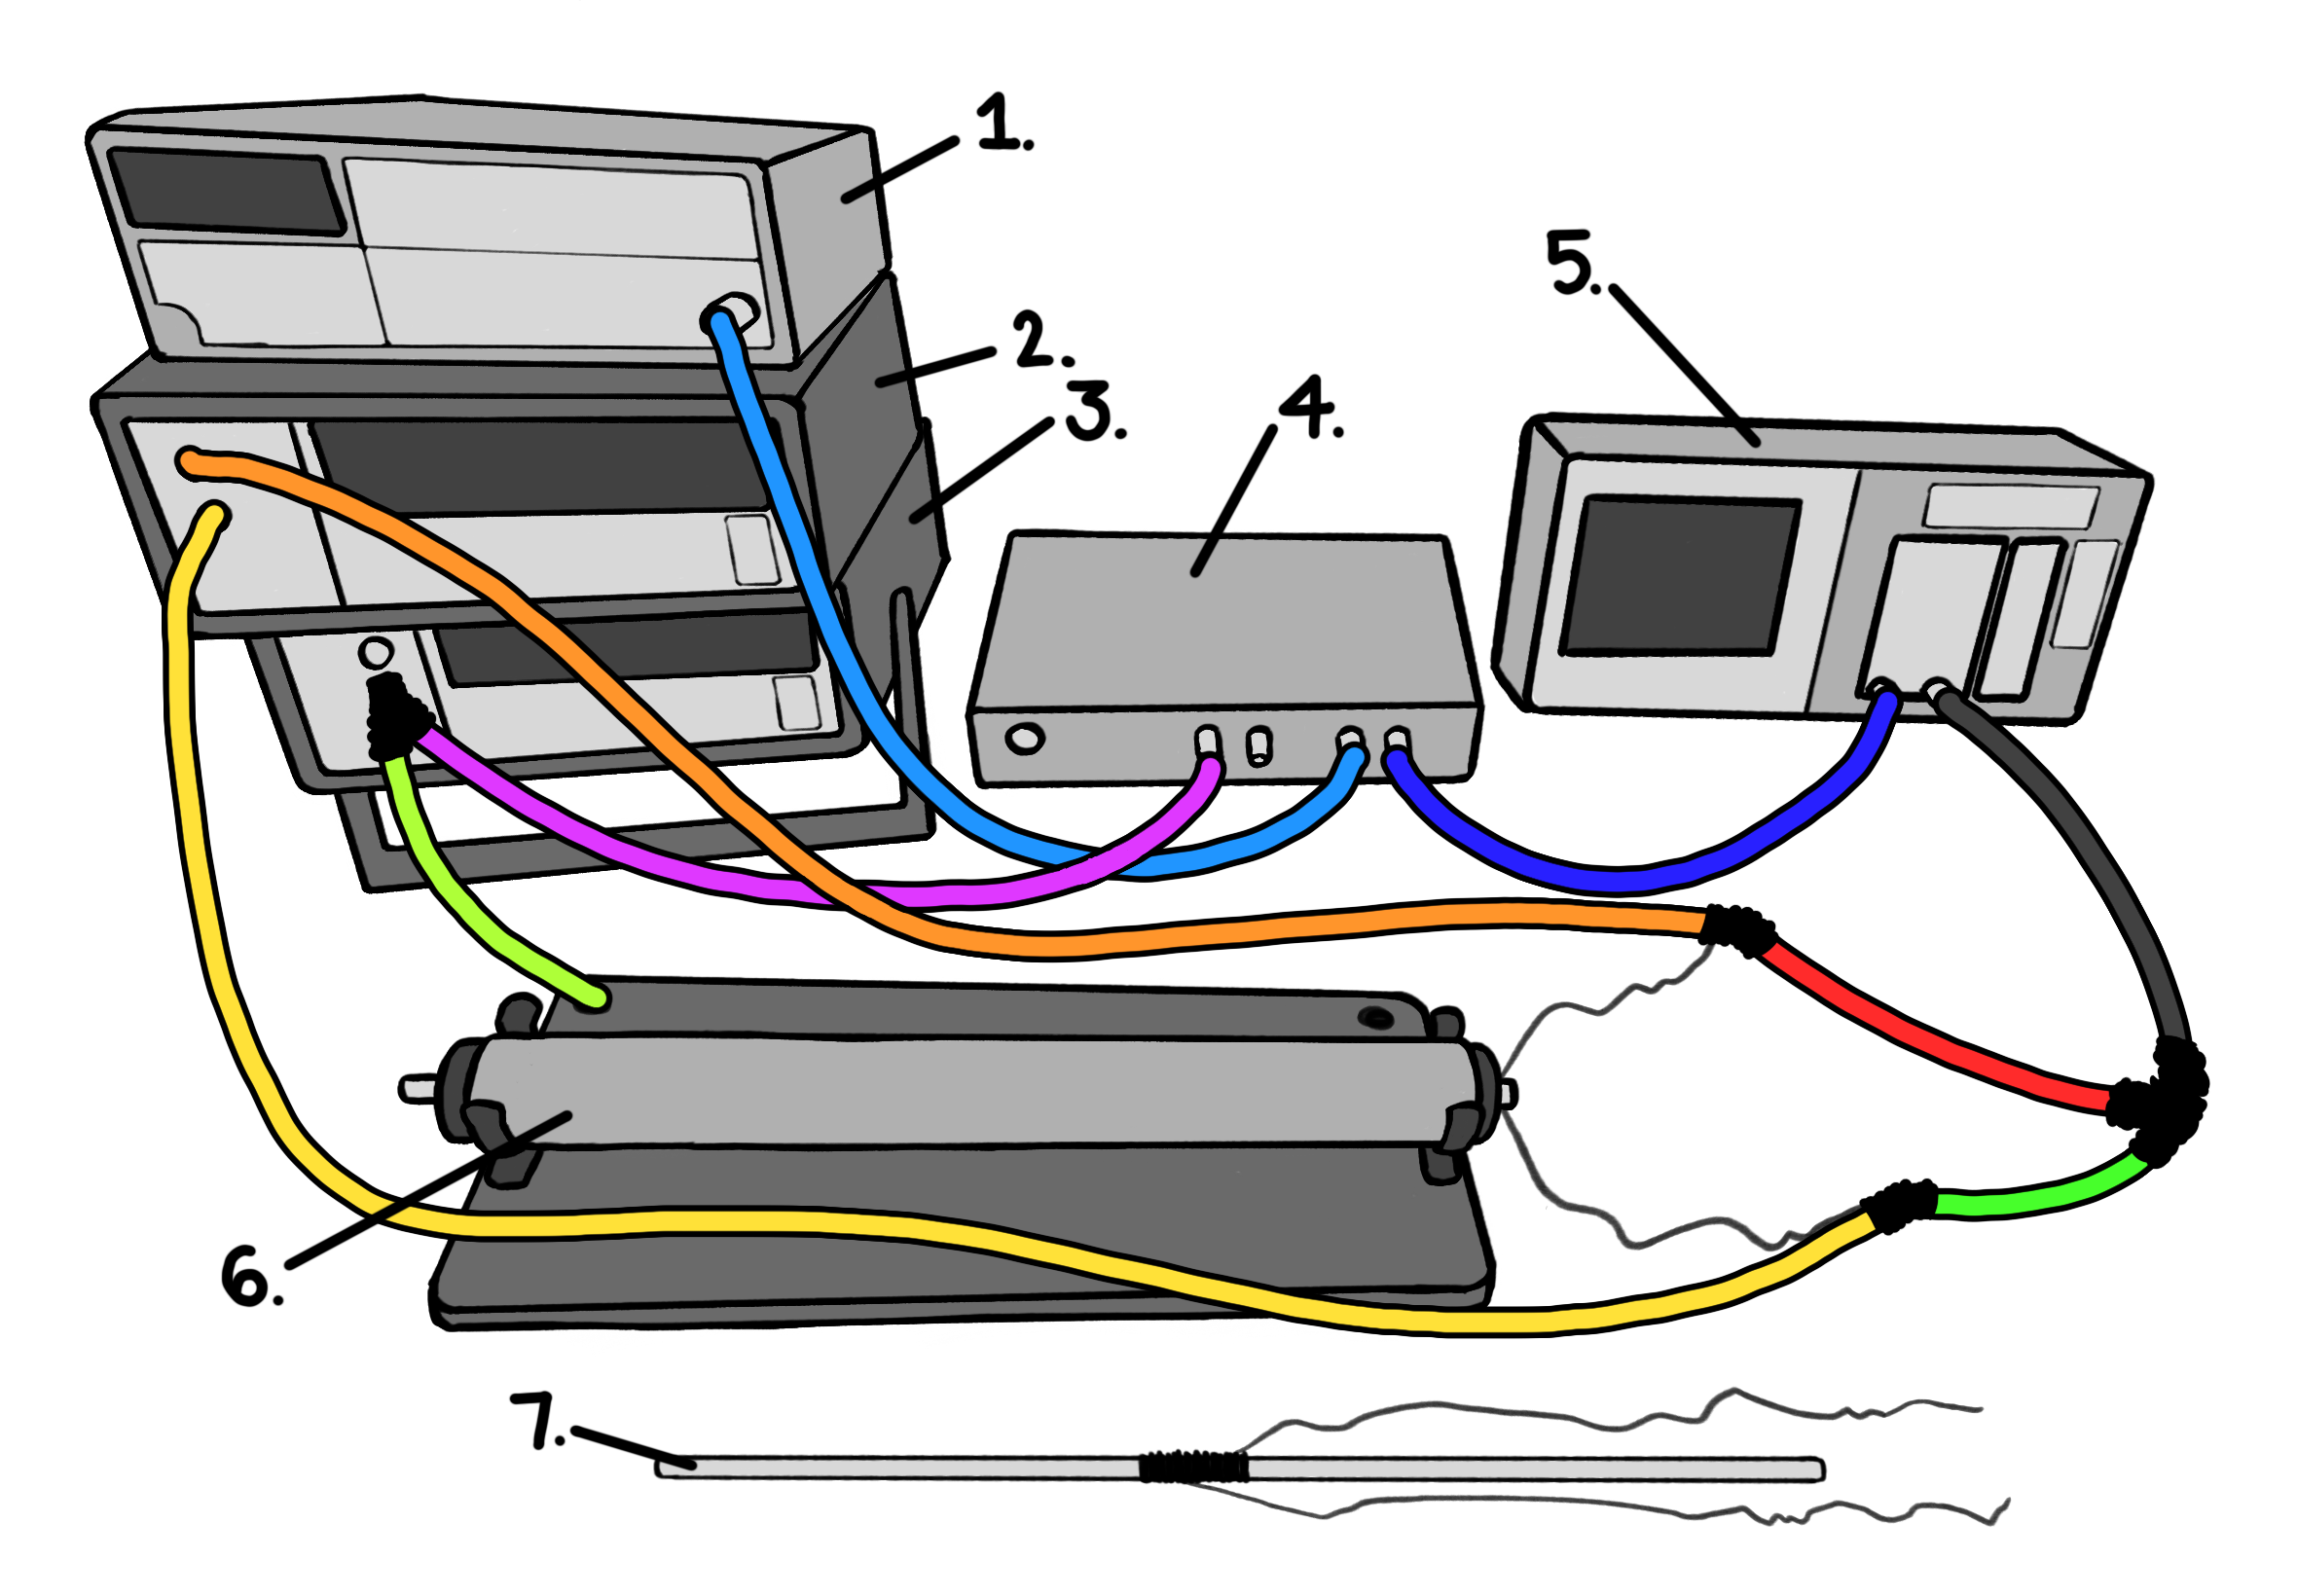
\includegraphics[width=\linewidth]{skindepth_exp.png}
  \caption{Experimental setup wire connections; \textit{1. frequency generator, 2. digital multimeter (voltmeter), 3. digital multimeter (ammeter), 4. voltage amplifier, 5. oscilloscope, 6. solenoid, 7. metal rod (brass, aluminium, copper, or steel)}}
  \label{fig:1}
\end{figure}

\begin{figure}[ht]
  \centering
  \resizebox{0.6\linewidth}{!}{%
  \begin{circuitikz}
    \tikzstyle{every node}=[font=\large]
    \draw (3.75,17) to[rmeter, t=A] (5.25,17);
    \draw (5.25,17) to[L,l={ \large N1} ] (7.75,17);
    \draw (7.75,17) to[short] (9.25,17);
    \draw (9.25,17) to[short] (9.25,18.75);
    \draw (3.75,18.75) to[sinusoidal voltage source, sources/symbol/rotate=auto,l={ \large Sine Source (V)}] (9.25,18.75);
    \draw (3.75,18.75) to[short] (3.75,17);
    \draw (3.75,14.5) to[rmeter, t=V] (9.25,14.5);
    \draw (3.75,16.25) to[short] (3.75,14.5);
    \draw (9.25,16.25) to[short] (9.25,14.5);
    \draw (9.25,16.25) to[L,l={ \large L2 ($\mu$H)} ] (3.75,16.25);
  \end{circuitikz}
  }%
\caption{Circuit diagram of the skin depth experiment setup.}
\label{fig:2}
\end{figure}

The solenoid was connected to a sine wave (alternating current) function generator with varying frequencies. The metal rods of brass, aluminium, copper, and steel (separately) were inserted inside of the solenoid and the time-varying magnetic field penetrates the materials, generating a time-varying magnetic field.

A secondary pick-up coil of 500 turns was wrapped around the middle of each of the metal rods. The magnetic field generated inside of the solenoid induced a voltage through the metal rod, which was measured by the pick-up coil. The ends of the wire used for this coil were clamped to an oscilloscope to measure the time lag between the applied voltage and the induced voltage which was used to determine the phase shift, and clamped also to a digital multimeter measuring the induced voltage.

The current through the solenoid was kept constant at 19 ± 0.1 mA, ensuring a consistent magnetic field was generated for each metal and necessarily low to avoid overheating elements that could affect science readings, and the frequency was taken from 5 to 62 kHz in steps of 3 kHz.

Frequency, pick-up voltage, and time lag between the oscilloscopes peak-to-peak readings were all noted, from which the $V/f$ ratio and phase shift could be calculated. With these values, two independent measurements and graphs of the skin depth could be made.

\subsection{Calculating Permeability of Steel}

As was seen in \autoref{eq:2} in the $R \gg \delta$ limit, the experimental setup introduces a series of constants. One of the metals, copper in this instance, can be taken for its conductivity (found in the first part of the experiment), and a relative permeability $\mu_r$ of approximately 1 can be assumed for copper, aluminium, and brass. Two apparatus constants $G$, $H$ were defined:

The \textbf{voltage constant ($G$)} was calculated from the slope ($a_{V,Cu}$) of the $V/f$ vs. $f^{-1/2}$ plot,

\vspace{-1.5ex}
\begin{equation*}
  \frac{V}{f} = G \times \sqrt{\frac{\mu_r}{\sigma}} f^{-1/2}
\end{equation*}

From the relationship $V/f \propto f^{-1/2}$, $G$ can then be found to be the coil's voltage sensitivity:

\vspace{-1.5ex}
\begin{equation} \label{eq:3}
  \begin{aligned}
  a_{V,Cu} &= G \times \frac{1}{\sqrt{\sigma_{Cu}}} \\
  \implies G &= a_{V,Cu} \sqrt{\sigma_{Cu}}
  \end{aligned}
\end{equation}

The \textbf{phase constant ($H$)} can be similarly calculated from the slope ($a_{\phi,Cu}$) of the phase shift in radians $\phi$ vs. $\sqrt{f}$ plot,

\begin{equation*}
  \phi = H \times \sqrt{\mu_r \sigma} \times \sqrt{f}
\end{equation*}

As the phase shift is also relative to the frequency, $H$ can be found to be the geometry's phase sensitivity:

\vspace{-1.5ex}
\begin{equation} \label{eq:4}
  \begin{aligned}
  a_{\phi,Cu} &= H \times \sqrt{\sigma_{Cu}} \\
  \implies H &= \frac{a_{V,Cu}}{\sqrt{\sigma_{Cu}}}
  \end{aligned}
\end{equation}

The conductivity of the steel rod can be found with the ratio of the two slopes removes the permeability dependence:

\vspace{-1.5ex}
\begin{equation} \label{eq:5}
  \begin{aligned}
  \frac{a_{\phi,Cu}}{a_{V,Cu}} &= \frac{H \sqrt{\mu_r \sigma}}{G \sqrt{\frac{\mu_r}{\sigma}}} = \frac{H}{G} \sigma \\
  \sigma_{\text{steel}} &= \left( \frac{a_{V,Cu}}{a_{\phi,Cu}} \right) \times \left( \frac{G}{H} \right)
  \end{aligned}
\end{equation}

Similarly, the permeability of the steel rod can be found by multiplying the two slopes to remove the conductivity dependence:

\vspace{-1.5ex}
\begin{equation} \label{eq:6}
  \begin{aligned}
    a_{\phi,Cu}\cdot{a_{V,Cu}} &= \left( G \sqrt{\frac{\mu_r}{\sigma}} \right) \left( H \sqrt{\mu_r \sigma} \right) = G H \mu_r \\
    \mu_{r,\text{steel}} &= \frac{a_{\phi,Cu}\cdot{a_{V,Cu}}}{G \cdot H}
  \end{aligned}
\end{equation}

\section{Results} \label{sec:4}

\subsection{Skin Depth with Voltage}

The values of the $V/f$ ratio were plotted against the inverse square root of the frequency for the range of frequencies observed, seen in \autoref{fig:A1}. At much higher frequencies, the generated magnetic field penetrates the material more easily, observed as a valley in the values for which the skin effect phenomenon breaks down.

At certain ranges of frequency, the skin effect is best seen with its discussed linearity, shown in \autoref{fig:3}. For all metals except copper, the linear fit line is observed to agree very well with the data.

\begin{figure}[H]
  \centering
  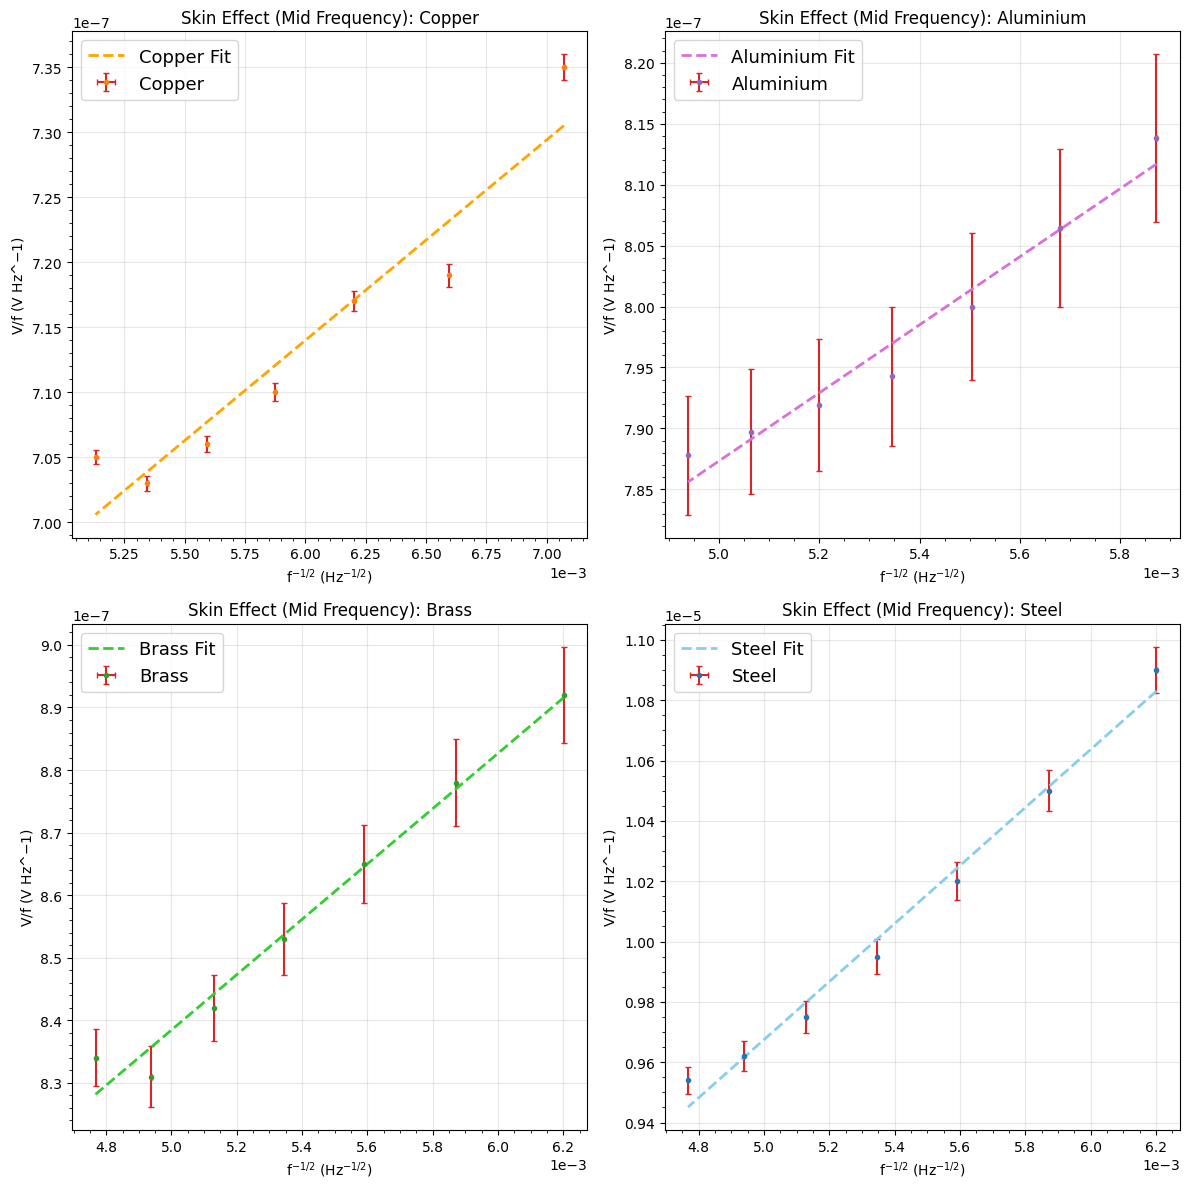
\includegraphics[width=.95\linewidth]{skindepth_mf.png}
  \caption{Skin effect clipped at mid-range frequencies.}
  \label{fig:3}
\end{figure}

\vspace{-2ex}
The values of the slopes for each metal were taken and shown in \autoref{tab:1}, which were then used to calculate the conductivities.

\begin{table}[H]
\centering
\caption{Table of the slope values obtained for each metal rod from \autoref{fig:3}.}
\label{tab:1}
  \begin{tabular}{|
  >{\columncolor[HTML]{EFEFEF}}c |c|}
  \hline
  Metal     & \cellcolor[HTML]{EFEFEF}Slope ($a$) \\ \hline
  Copper    & \num{1.54e-5}                           \\ \hline
  Aluminium & \num{2.79e-5}                          \\ \hline
  Brass     & \num{4.42e-5}                          \\ \hline
  Steel     & \num{9.61e-4}                          \\ \hline
  \end{tabular}
\end{table}

\subsection{Conductivity Calculations}

The proportionality of the skin depth had been established as $V/f \propto 1/\sqrt{\sigma}$, which can be used in tangent with the skin depth formula in \autoref{eq:1} to give a way to calculate the conductivity of the metals based on the slope of the linear fit line. Results of these calculations are given in \autoref{tab:2}.

\begin{table}[H]
\centering
\caption{Table of calculated the conductivity for each metal rod.}
\label{tab:2}
\resizebox{.99\linewidth}{!}{
  \begin{tabular}{|
  >{\columncolor[HTML]{EFEFEF}}c |c|c|}
  \hline
  Metal     & \cellcolor[HTML]{EFEFEF}Calculated (S/m) & \cellcolor[HTML]{EFEFEF}Expetected (S/m) \\ \hline
  Copper    & (5.31 ± 1.58) $\times$\num{e7}                         & \num{5.96e7}                                   \\ \hline
  Aluminium & (1.62 ± 0.34) $\times$\num{e7}                         & \num{3.77e7}                                   \\ \hline
  Brass     & (6.46 ± 1.12) $\times$\num{e6}                          & \num{1.59e7}                                  \\ \hline
  \end{tabular}
}
\end{table}

While the values calculated and obtained from this experiment do not align with the expected values, the expected relationship of \textit{Copper} $>$ \textit{Aluminium} $>$ \textit{Brass} with respect to electrical conductivity is observed, also seen in \autoref{fig:A2}.

A conductivity was not able to be obtained for the steel rod using this method due to its high relative permeability as a likely ferromagnet.

\subsection{Skin Depth with Phase Shift}

The time lag between the voltage and the induced voltage was measured and used to find the phase shift $\phi$, which was plotted against the square root of the frequency as the relationship demands, shown in \autoref{fig:4}.

\begin{figure}[H]
  \centering
  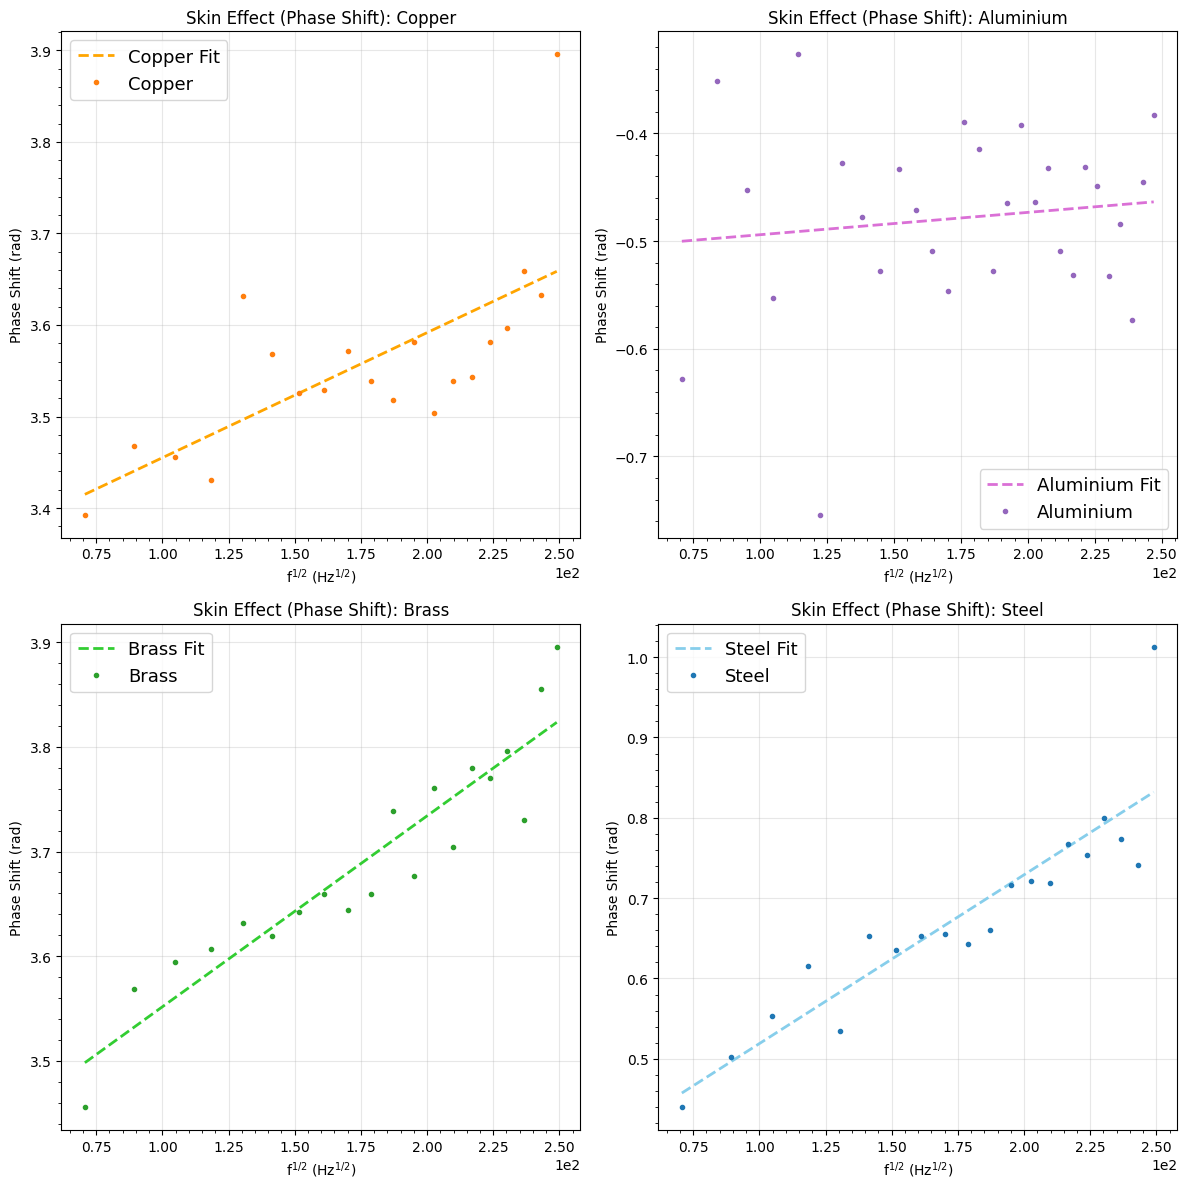
\includegraphics[width=.95\linewidth]{se_phase.png}
  \caption{Skin effect with the phase shift in radians.}
  \label{fig:4}
\end{figure}

Despite the scattered frequencies of the aluminium plot, the skin effect can still be observed in the other metal rods with the same linear relationship.

\subsection{Permeability Calculation}

The conductivity and relative permeability of the steel rod made use of \autoref{eq:5} and \autoref{eq:6}, and the slopes of the lines of linear fit for both the voltage and phase shift plots. The following results were obtained:

\begin{itemize}
  \item[] \textbf{Conductivity} ($\sigma$): \num{1.31e6} S/m
  \item[] \textbf{Relative permeability} ($\mu_r$): \num{95.90}
\end{itemize}

While low values for a ferromagnetic steel, these values could indicate at a carbon steel rod or an alloy steel rod.

\section{Analysis and Discussion} \label{sec:5}

The results of this experiment observing the behaviour of the skin effect on cylindrical conductors aligned well with the theoretical expectations discussed. For all materials copper, aluminium, brass, and steel, the relationship between the induced voltage ratio $V/f$ and the inverse square root of the frequency $f^{-1/2}$ showcased the linearity expected for the "strong skin effect" limit ($R \gg \delta$). This linear relationship was best observed in a mid-range of frequencies, shown in \autoref{fig:3}. At higher frequencies, the values began to deviate from the linear fit to form a valley at which the skin effect phenomenon began to break down as the generated magnetic field penetrated the material more easily, seen in \autoref{fig:A1}.

\subsection{Conductivity of the Non-Magnetic Materials}

The calculated conductivity for the copper rod was found to be (5.31 ± 1.58) $\times$\num{e7} S/m and aligns closely with the expected value of \num{5.96e7} S/m as the expected literature value falls within the uncertainty range. This result validates the skin depth formula derived from Faraday's law.

For aluminium and brass, however, showed significant discrepancies from the literature values despite maintaining the correct order of \textit{Copper} $>$ \textit{Aluminium} $>$ \textit{Brass}, which shows the experimental method successfully captured the expected physical trend. Both values for the metals were much lower than the expected values by about 57\% and 59\% for aluminium and brass respectively. A reason for this discrepancy could likely be attributed to the possibility of these metal rods being alloys instead of pure metal, which tend to have lower conductivities in comparison.

Another reason for errors in calculation could be improper values, particularly in the number of turns for both the solenoid and the pick-up coil, which were taken directly from the provided manual and may not align with the apparatus used. The constant current of 19 ± 0.1 mA was also critical, though more precise current values or perhaps lower current could have influenced the results positively. Additionally, the "strong skin depth" assumption (also called "thin skin") may not be as applicable to a metal like brass, which has lower conductivity and therefore greater skin depth.

\subsection{Conductivity and Permeability of Steel}

Due to its high relative permeability, the standard calculations used for the other metal rods was not applicable to steel. A set of decoupling equations were used alongside the slopes from the voltage graph ($a_V$) and the phase graph ($a_{\phi}$) to cancel out the unknown variables and isolate the variables of interest. With this method, a resulting conductivity of \num{1.31e6} S/m and relative permeability of 95.90 were obtained for the steel sample, which align well with a lower ferromagnetic steel-type, such as a carbon or alloy steel material.

Compared to the voltage measurements obtained from the digital multimeter, the phase shift measurements showed to be more prone to experimental errors and uncertainties. As was seen in the aluminium plot, data was more scattered than the other plots, which might suggest noise or difficulty in timing the peak-to-peak lag on the oscilloscope with a manual cursor, which may have introduced noise into the $H$ constant and thus into the subsequent steel calculations.

\section{Conclusion}

This experiments successfully demonstrated the principles of the skin depth phenomenon and how, at high frequencies, the depth of penetration of the magnetic field gets confined to the surface of a cylindrical conductor as a "skin". The linear behaviour predicted for the strong skin effect limit ($R \gg \delta$) was observed at mid-range frequencies for all tested materials, and the slopes of these linear fit lines were successful in calculating conductivity values for the three non-magnetic metals. While copper results agreed with the expected literature values and were within the calculated uncertainty, the values for aluminium and brass deviated from literature. These deviations may likely arise from the possibility of the materials being alloys and the limitations of the "thin-skin" limit assumption for metals of lower conductivities.

A decoupling method making use of the graph relationships and similar linear fits in a phase shift graph were used to determine the conductivity and permeability of the steel sample rod as it showcased ferromagnetic behaviour in the voltage graphs. It was successful in separating the variable parameters, and based on the values obtained from the calculations it can be presumed that the sample used may have been a light carbon steel or alloy steel metal given its comparatively low relative permeability of 95.90.

Overall, this experiment verified the frequency-dependent nature of magnetic penetration in conductors via the electromagnetic phenomenon of the skin depth.

%%%%%%%%%%%%%%%%%%%%

% References - switch to single column
\onecolumn

\bibliographystyle{IEEEtran}
\bibliography{PHYC30170References} \label{sec:ref}

\newpage

% Appendix - single column
\section*{Appendix} \label{sec:A}
\addcontentsline{toc}{section}{Appendix}

\subsection*{Figures}
\addcontentsline{toc}{subsection}{Figures}

\begin{figure}[H]
  \centering
  
\includegraphics[width=.65\textwidth]{skindepth.png}
  \caption{Skin depth for all frequencies observed.}
  \label{fig:A1}
\end{figure}

\begin{figure}[H]
  \centering
  \begin{subfigure}{.49\textwidth}
    \centering
    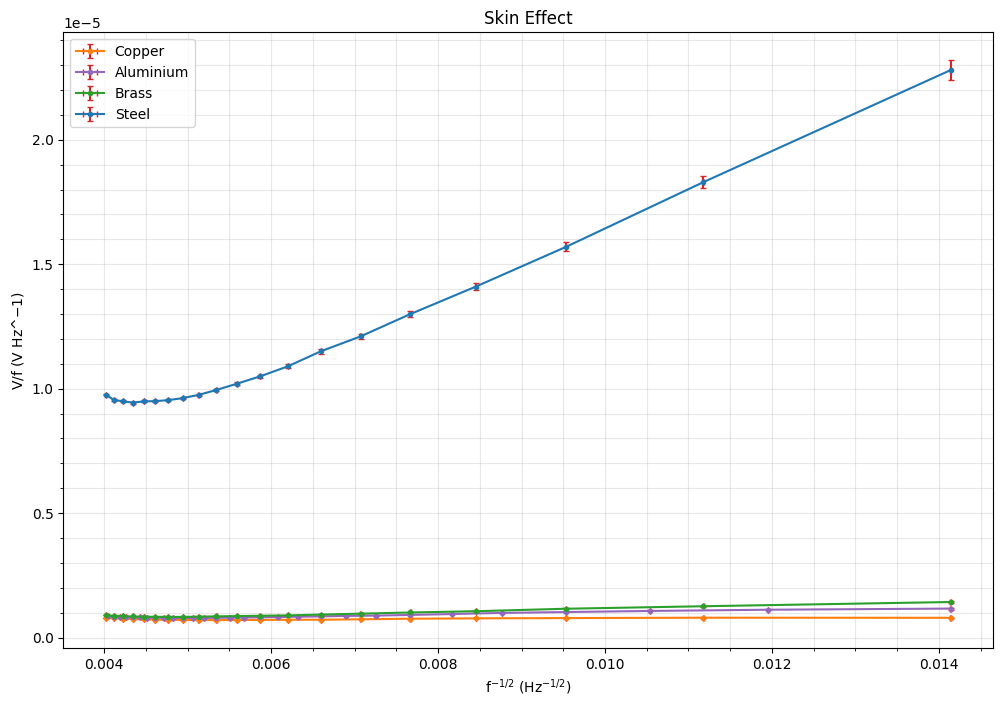
\includegraphics[width=\linewidth]{se_all.png}
    \subcaption{All metals (full range)}
  \end{subfigure}
  \begin{subfigure}{.49\textwidth}
    \centering
    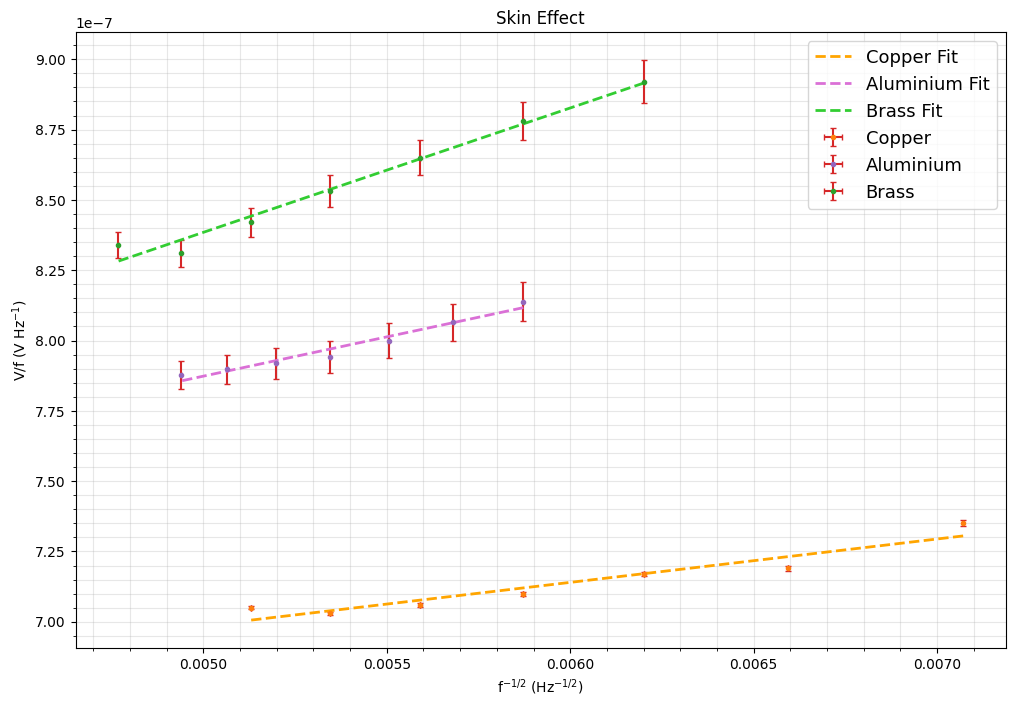
\includegraphics[width=\linewidth]{se_metals.png}
    \subcaption{Copper, Aluminium, Brass (mid-range)}
  \end{subfigure}
  \caption{Single skin depth plots of all four metals observed; copper, aluminium, brass, steel.}
  \label{fig:A2}
\end{figure}

\addcontentsline{toc}{subsection}{Code}


\includepdf[pages={1,3,5-7,9-15}]{skindepth.pdf}

\end{document}